\documentclass[11pt,a4paper]{article}
\usepackage[margin=2.5cm]{geometry}
\usepackage{graphicx}
\usepackage{booktabs}
\usepackage{array}
\usepackage{amsmath}
\usepackage{float}
\usepackage{subcaption}
\usepackage[hidelinks]{hyperref}

\setlength{\emergencystretch}{1.5em}

% Float placement: allow large figures and tables on text pages,
% and put any page made only of floats at the top instead of centring it
\renewcommand{\topfraction}{0.9}
\renewcommand{\bottomfraction}{0.8}
\renewcommand{\textfraction}{0.07}
\renewcommand{\floatpagefraction}{0.8}
\makeatletter
\setlength{\@fptop}{0pt}
\makeatother

\newcommand{\high}{$>$50K}
\newcommand{\low}{$\leq$50K}

\title{Predicting Income from Census Data:\\ A Supervised Learning Proof-of-Concept}
\author{Group members: [Names]}
\date{\today}

\begin{document}
\maketitle

\noindent\textbf{Dataset used:} Adult / Census Income (OpenML, \texttt{name="adult"}, version~2).

%=====================================================================
\section{Problem Framing and Exploratory Data Analysis}
%=====================================================================

\subsection{Task and train/test split}
The task is to predict whether an individual earns more than \$50{,}000 per year from 14
demographic and employment attributes of the 1994 US Census \cite{kohavi1996}. The
positive class (\high{}) represents 23.9\% of the observations, so the problem is
imbalanced (Section~\ref{sec:imbalance}).

The data are split once into a training set (80\%, 39{,}032 rows) and a test set (20\%,
9{,}758 rows), with stratification on the target and a fixed seed; both sets contain
23.9\% of positives. The test set is not used before the final evaluation: model
comparisons rely on 5-fold stratified cross-validation within the training set, and every
relationship between a feature and the target reported below is computed on the training
set only.

\subsection{Data quality}

\paragraph{Duplicates and removed columns.}
The raw data contain 48{,}842 rows, of which 52 are exact duplicates; these are removed,
leaving 48{,}790 observations. This is done before dropping any column: if \texttt{fnlwgt}
were removed first, 6{,}374 rows would appear duplicated, although they are distinct
individuals who share the same profile, not recording errors. Two columns are then
removed. \texttt{fnlwgt} is a sampling weight indicating how many people in the US
population a respondent represents; it is not linked to the individual's
characteristics. \texttt{education\_num} maps one-to-one onto \texttt{education} and is
therefore redundant.

\paragraph{Missing values.}
Three columns contain missing values: \texttt{workclass} (5.7\%), \texttt{occupation}
(5.7\%) and \texttt{native\_country} (1.8\%). 10 rows with no occupation belong to the
\texttt{Never-worked} class, so they have no occupation by definition. Then we have 2,795 rows where both \texttt{workclass} and \texttt{occupation}
are missing together.

To choose how to handle them, we need to know whether these values are missing at random
\cite{rubin1976}. We cannot know why a value is missing, but we can
compare people with and without a reported work class (Table~\ref{tab:missing}).

\begin{table}[htbp]
\centering
\caption{Profile of people with a missing or reported work class (training set).}
\label{tab:missing}
\small
\begin{tabular}{lcc}
\toprule
 & Work class missing & Work class reported \\
\midrule
Aged 20 or younger, or 65 or older & 39.2\% & 9.9\% \\
Works less than 35 hours per week   & 44.7\% & 15.6\% \\
Lives with parents (\texttt{Own-child}) & 30.4\% & 14.7\% \\
Earns \high{}                        & 9.4\%  & 24.8\% \\
Earns \high{}, aged 21 to 64 only    & 10.9\% & 26.7\% \\
\bottomrule
\end{tabular}
\end{table}

People with a missing work class are much more often very young or old, work part time
more often, and more often live with their parents. This profile suggests people outside
regular employment, such as students and retirees. As a result, they earn \high{} much
less often (9.4\% against 24.8\%). Even among people aged 21 to 64, the gap remains (10.9\%
against 26.7\%), so age alone does not explain it. The missing values of
\texttt{workclass} and \texttt{occupation} are therefore not random: their absence is probably
linked to the person's situation and to income.

The case of \texttt{native\_country} is different. People with a missing country earn
\high{} in 25.1\% of cases, close to the overall rate of 23.9\%. Their absence does not
seem linked to the person's situation.

\paragraph{Extreme values.}
We examined the four numerical variables in two ways: a standard outlier rule and the
maximum values.

First, we applied Tukey's rule that flags values below $Q_1 - 1.5\,\mathrm{IQR}$ or above
$Q_3 + 1.5\,\mathrm{IQR}$. For age, the rule
flags 0.4\% of people, all older than 78. These are real elderly people, not errors. For
weekly hours, it flags 27.6\% of people. This happens because 46.7\% of people work
exactly 40 hours, so $Q_1 = 40$, $Q_3 = 45$, and the bounds are 32.5 and 52.5 hours. As
Figure~\ref{fig:eda}b shows, the rule then flags wrongly normal part-time jobs and long working
weeks. Regarding capital income, most values are zero (91.7\%
for gains and 95.3\% for losses). Therefore, $Q_1 = Q_3 = 0$ and every non-zero value would be
flagged. The non-zero values are also very skewed (handled in section 2.2): the median gain is 7{,}298, but the
maximum is 99{,}999 (Appendix~\ref{app:figures}).

Second, the maximum values show that some variables are capped. 54 people are exactly 90
years old, against 6 and 2 for ages 88 and 89. 137 people work exactly 99 hours per week.
244 people have a capital gain of exactly 99{,}999, while the next highest gain is
41{,}310. These values probably mean ``this amount or more'' and are not errors. For instance, the
99{,}999 value is very informative: 100\% of these people earn \high{}.

\paragraph{Rare and inconsistent categories.}
Some categories contain very few people. In the training set, \texttt{Never-worked} has 8
people, \texttt{Without-pay} 20 and \texttt{Armed-Forces} 12. In the full dataset, 17
countries have fewer than 50 people. Rates computed on such small groups are unreliable.
We also found four inconsistent rows: one woman is recorded as a \texttt{Husband} and
three men as a \texttt{Wife}.

\subsection{Relationships with the target}

\begin{figure}[htbp]
\centering
\begin{subfigure}{0.49\linewidth}
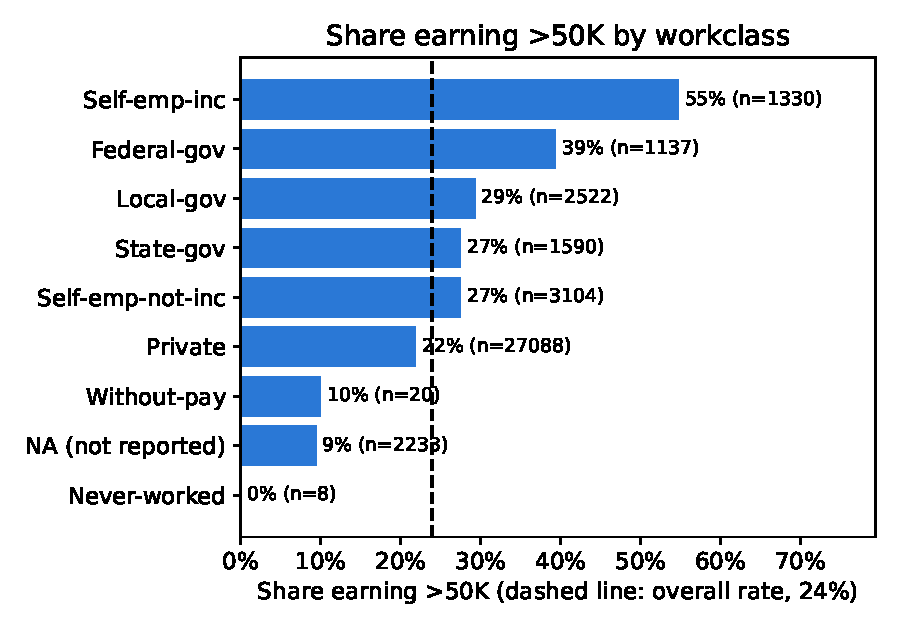
\includegraphics[width=\linewidth]{figures/rate_workclass.pdf}
\caption{Share of \high{} by work class}
\end{subfigure}
\hfill
\begin{subfigure}{0.49\linewidth}
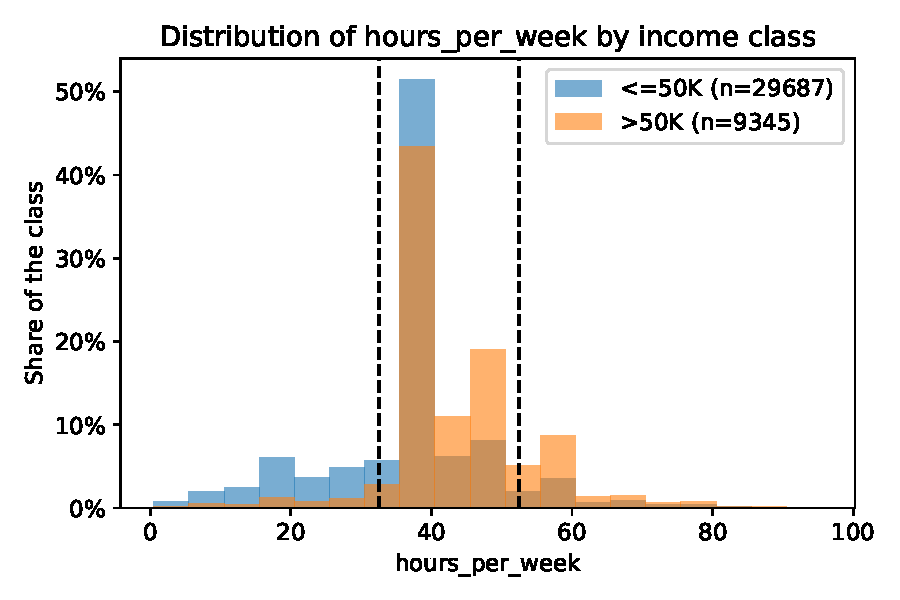
\includegraphics[width=\linewidth]{figures/hist_hours_per_week.pdf}
\caption{Weekly hours by class}
\end{subfigure}

\medskip
\begin{subfigure}{0.49\linewidth}
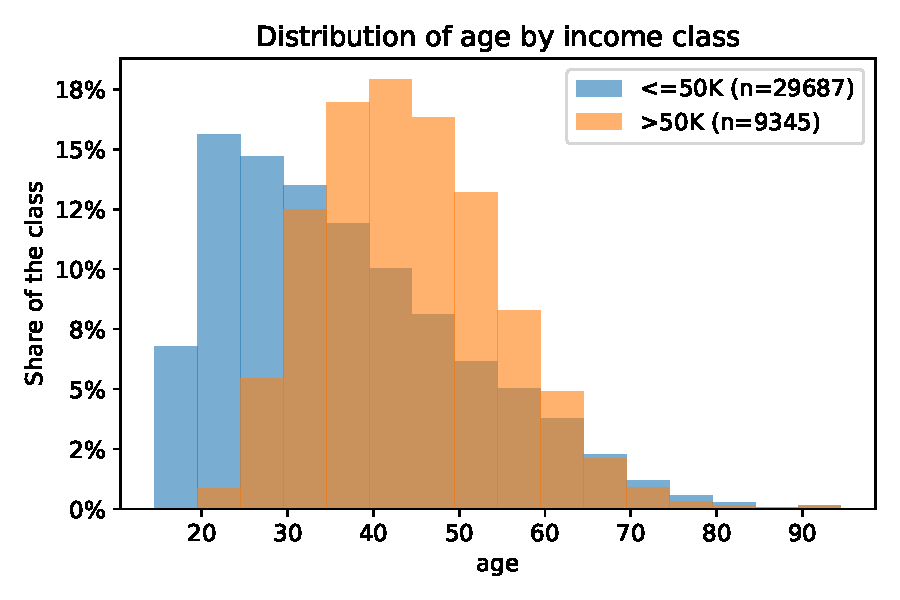
\includegraphics[width=\linewidth]{figures/hist_age.pdf}
\caption{Age by class}
\end{subfigure}
\hfill
\begin{subfigure}{0.49\linewidth}
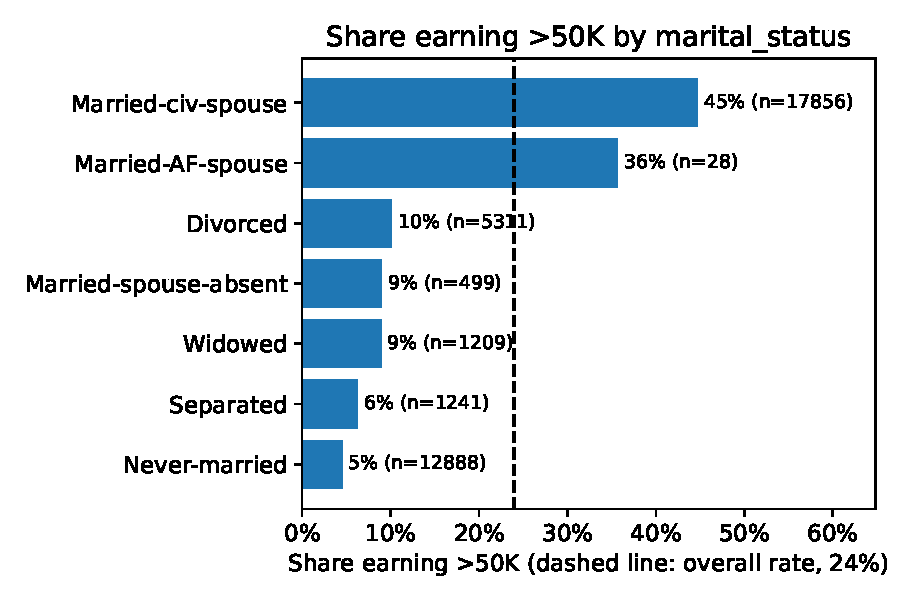
\includegraphics[width=\linewidth]{figures/rate_marital_status.pdf}
\caption{Share of \high{} by marital status}
\end{subfigure}
\caption{Exploratory analysis on the training set. (a) and (d): share of people earning
\high{} in each category; the dashed line is the overall rate. In (a), missing work
classes are shown as a separate bar. (b) and (c): distribution within each class (each
class sums to 100\%). In (b), the dashed lines are Tukey's bounds:
$40 - 1.5 \times 5 = 32.5$ and $45 + 1.5 \times 5 = 52.5$ hours.}
\label{fig:eda}
\end{figure}

\paragraph{Employment.}
Income varies strongly with the type of employment (Figure~\ref{fig:eda}a). The private
sector covers 69\% of people, and 22\% of them earn \high{}. The rate is higher for
federal employees (39\%) and highest for self-employed people with their own company
(55\%). People with a missing work class have a low rate (9\%), in line with the profile
of Table~\ref{tab:missing}. Working time also matters (Figure~\ref{fig:eda}b): 40.2\% of
people who work more than 40 hours earn \high{}, against 9.4\% of people who work less
than 40 hours.

\paragraph{Demographics.}
High earners are older: their median age is 43, against 34 for the others
(Figure~\ref{fig:eda}c), and almost no one under 25 earns \high{} (1.2\%). Marital status
also matters. Married people living with their spouse earn \high{} in 44.7\% of cases,
while the other frequent statuses stay between 4.5\% and 10.1\% (Figure~\ref{fig:eda}d).
Education shows a similar gap, from 1.6\% (\texttt{Preschool}) to 74.1\%
(\texttt{Doctorate}). Finally, 21.3\% of high earners have a capital gain, against 4.1\%
of the others.

\paragraph{Sex.}
The share of high earners differs by sex: 30.3\% for men against 11.1\% for women. In
addition, \texttt{relationship} is closely linked to sex: a \texttt{Husband} is a man in
all cases but one, and a \texttt{Wife} is a woman in all cases but three. This link will be important for our fairness audit.

%=====================================================================
\section{Data Preparation and Feature Engineering}
%=====================================================================

\subsection{Missing values}
Section~1.2 showed that the missing values of \texttt{workclass} and \texttt{occupation}
are not random. We considered three options. Deleting these rows would remove 5.7\% of
the data and, above all, a specific group of low earners, which would bias the model.
Replacing them with the most frequent value (\texttt{Private}) would mix two groups with
different incomes (9.4\% against 21.9\%). We therefore keep them as a separate category,
called \texttt{Missing}, in both columns. The model can then learn what the absence means.

For \texttt{native\_country}, the share of high earners (25,1\%) is similar to the overall share (23,9\%), 
which suggests that this missingness is unrelated to the target, and it concerns only 1.8\% of rows. 
We therefore replace these values with the most frequent country, the United States,
which covers 91.4\% of people whose country is known. It is the most likely value, so the
risk of error is small. 

Both treatments are applied inside the pipeline: the most
frequent value is computed on the training folds only, so no information comes from the
data used for evaluation.

\subsection{Extreme values}
We do not remove any extreme value, for two reasons: none of them is an error and
removing them would lose information, especially the capital gain of 99{,}999, which
always means \high{}.

The remaining question is whether these values can harm the models. Tree-based models are
not affected, because they split the data with thresholds. The logistic regression is more sensitive so for this model, numerical features are standardised and capital
income is log-transformed (Section~\ref{sec:features}), which reduces the weight of very
large values.

\subsection{Rare and inconsistent categories}
Regarding the rare categories, we keep them. Most of them disappear in the engineered
features of Section~\ref{sec:features}: rare countries are grouped in
\texttt{native\_us}, and \texttt{Married-AF-spouse} is merged into \texttt{is\_married}.
The others, such as \texttt{Never-worked}, are too small to influence the models.
Regarding the four inconsistent rows, we also keep them. They represent less than 0.01\%
of the data and cannot affect the results, while correcting them would
require guessing which value is wrong.

\subsection{Encoding and scaling}
Models need numerical inputs. The six categorical variables have no natural order, so we
use one-hot encoding: each category becomes a 0/1 column. This concerns
\texttt{workclass}, \texttt{education}, \texttt{occupation}, \texttt{relationship},
\texttt{race} and \texttt{sex}. Very rare categories not seen during training are ignored in the encoder. 
We keep one column per category. Although this
creates one redundant column per variable, it is not a problem: the logistic
regression uses L2 regularisation by default, and trees are not affected. Numerical
features are standardised. All models use the same pipeline, so that
Section~\ref{sec:models} compares the models only.

\subsection{Engineered features}
\label{sec:features}
We create three features, each replacing raw columns (Table~\ref{tab:features}).

\begin{table}[htbp]
\centering
\caption{Engineered features and the columns they replace.}
\label{tab:features}
\small
\begin{tabular}{>{\raggedright\arraybackslash}p{2.0cm}>{\raggedright\arraybackslash}p{2.6cm}>{\raggedright\arraybackslash}p{3.5cm}>{\raggedright\arraybackslash}p{5.9cm}}
\toprule
Feature & Replaces & Definition & Justification \\
\midrule
\texttt{capital\_net} & \texttt{capital\_gain}, \texttt{capital\_loss} &
$\operatorname{sign}(g-\ell)\log(1+|g-\ell|)$, with $g$ the gain and $\ell$ the loss &
No one has both a gain and a loss, so one column keeps all the information. The log
reduces the skew (Appendix~\ref{app:figures}). \\
\addlinespace
\texttt{is\_married} & \texttt{marital\_status} & 1 if married and living with spouse &
The income gap is concentrated in this group: 44.7\% against at most 10.1\% for the
other frequent statuses. \\
\addlinespace
\texttt{native\_us} & \texttt{native\_country} & 1 if born in the United States &
Most countries are too small for reliable rates, and the gaps between countries mostly
follow education (see below). \\
\bottomrule
\end{tabular}
\end{table}

Reducing \texttt{native\_country} to a binary \texttt{native\_us} indicator may appear to discard information. For instance,
5.1\% of people born in Mexico earn \high{}, against 42.9\% of people born in India. 
However, we still keep a single indicator for two reasons. First,
most countries are too small: 17 countries have fewer than 50 people, so their rates are
unreliable. Second, the gaps between countries mostly follow education. Across the 24
countries with at least 50 people, the share of high earners and the share of university
graduates (\texttt{Bachelors} or higher) have a correlation of 0.87. Since education is
already in the model, a detailed country variable would add little. The indicator still
keeps the main difference: 24.4\% of people born in the United States earn \high{},
against 18.4\% of the others. Note that this correlation is computed on country
averages, so it shows an association, not a causal link.

%=====================================================================
\section{Class Imbalance}
\label{sec:imbalance}
%=====================================================================

\subsection{Metrics}
The positive class represents only 23.9\% of the data. With such an imbalance, accuracy
is misleading: a model that always predicts \low{} reaches 76.1\% accuracy without finding
a single high earner. We therefore do not use accuracy, and choose metrics that focus on
the positive class.

Our main metric is the area under the precision--recall curve (PR-AUC). It measures how
well the model ranks high earners above the others, over all possible thresholds. It
focuses on the positive class, and a random model scores 0.239, the share of positives
\cite{saito2015}. We also report ROC-AUC, the standard ranking metric, but only as a
secondary metric. ROC-AUC relies on the false positive rate, $\mathrm{FP}/(\mathrm{FP} +
\mathrm{TN})$. Since true negatives are numerous, this rate stays low even when the model
makes many false alarms, so ROC-AUC can look better than the model really is. Our
imbalance is moderate, so this effect is smaller than in extreme cases, but it remains
visible: in Section~\ref{sec:models}, ROC-AUC is always much higher than PR-AUC.

Ranking metrics do not show the decisions the model actually makes. We therefore also
report three metrics at the default threshold of 0.5: recall, the share of high earners
that the model finds; precision, the share of predicted high earners that are correct;
and F1, which balances the two.

\subsection{Chosen remedy}
We handle the imbalance with class weighting. This method changes the training loss:
errors on high earners count more, so the model cannot ignore them. It does not change
the data and works inside the pipeline without any risk of leakage.

In the code, the weight is passed to each model as \verb|class_weight={0: 1, 1: w}|:
an error on a high earner counts $w$ times more than an error on a low earner. This is
equivalent to the \texttt{scale\_pos\_weight} parameter seen in class. We use
\texttt{class\_weight} because it is available in all three of our models, so the
imbalance is handled in the same way for each of them.

The best value of $w$ is not known in advance. We therefore treat it as a hyperparameter
and tune it with Optuna (Section~6), between 1 and $n_0/n_1 \approx 3.18$, where $n_0$
and $n_1$ are the numbers of negatives and positives in the training set. The lower
bound, $w = 1$, means no weighting: it leaves Optuna free to conclude that weighting is
not useful.

%=====================================================================
\section{Modelling Progression}
\label{sec:models}
%=====================================================================

\subsection{Evaluation protocol}
The goal of this section is to choose the model family, not its final settings. All
models therefore keep their default hyperparameters. Each model is placed in the same pipeline (Section~\ref{sec:pipeline})
and evaluated with 5-fold stratified cross-validation on the training set. The
training set is split into five parts that keep the class ratio. Each part is used once
for evaluation, while the model is trained on the other four. We report the mean score
over the five folds. To detect overfitting, we also compute the PR-AUC on the training
folds: a large gap with the cross-validated PR-AUC means that the model fits the training
data too closely.

\subsection{Models}
We compare three models of increasing flexibility.

\paragraph{Baseline: logistic regression.} It is a simple linear model, fast and easy to
interpret. It sets the minimum level that more complex models must beat.

\paragraph{Random forest.} It averages many decision trees, each trained on a random
sample of the data. Trees can capture non-linear effects and interactions between
features, and averaging them reduces the instability of a single tree.

\paragraph{Gradient boosting with LightGBM.} It builds trees one after another, each new
tree correcting the errors of the previous ones. Among boosting libraries, we chose
LightGBM over XGBoost and CatBoost. Our dataset is of moderate size and we have no strong
resource constraint, so raw performance does not clearly separate these libraries. Essentially, we chose LightGBM because it was
covered in class and because it accepts the same \texttt{class\_weight} parameter as the
scikit-learn models, so that the imbalance is handled identically for all models.

\subsection{Results}

\begin{table}[htbp]
\centering
\caption{Mean scores over 5-fold cross-validation on the training set (default
hyperparameters, threshold 0.5). The last column is the PR-AUC on the
training folds.}
\label{tab:models}
\small
\begin{tabular}{lcccccc}
\toprule
Model & Precision & Recall & F1 & ROC-AUC & PR-AUC & Train PR-AUC \\
\midrule
Logistic regression & 0.700 & 0.566 & 0.626 & 0.890 & 0.709 & 0.711 \\
Random forest       & 0.695 & 0.618 & 0.654 & 0.889 & 0.731 & 0.991 \\
LightGBM            & \textbf{0.781} & \textbf{0.658} & \textbf{0.714} & \textbf{0.929} & \textbf{0.830} & 0.860 \\
\bottomrule
\end{tabular}
\end{table}

\begin{figure}[htbp]
\centering
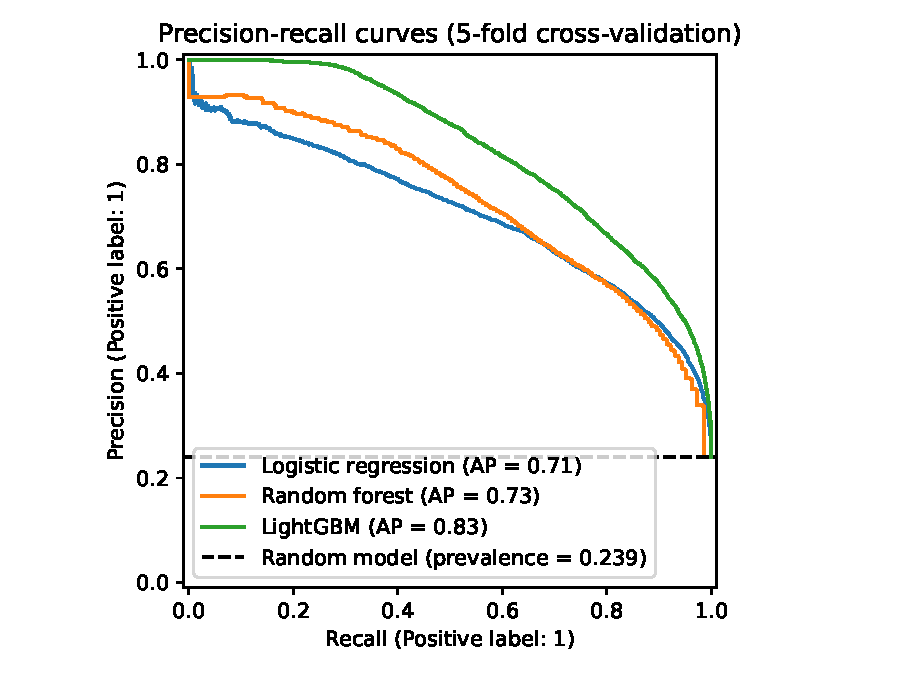
\includegraphics[width=0.6\linewidth]{figures/pr_curves.pdf}
\caption{Precision--recall curves from out-of-fold predictions (5-fold cross-validation
on the training set). AP is the average precision, i.e.\ the PR-AUC. The dashed line is
the score of a random model.}
\label{fig:pr}
\end{figure}

\paragraph{Ranking of the models.}
LightGBM is clearly the best model (Table~\ref{tab:models}). Its PR-AUC (0.830) is 12.1
points higher than the baseline, and it also has the best ROC-AUC, precision, recall and
F1. Figure~\ref{fig:pr} confirms this: its curve lies above the two others at almost every
level of recall. The random forest improves on the baseline only slightly (+2.2 points of
PR-AUC), and the two models have the same ROC-AUC (0.889 and 0.890). Their curves are
close, and they meet at high recall. All models are far above the random model (0.239),
so they all learn a real signal.

\paragraph{Overfitting.}
The gap between training and cross-validated PR-AUC differs strongly between models. The
logistic regression shows almost no gap (0.711 against 0.709). It does not overfit, but
its simple linear form limits its score. The random forest shows a very large gap (0.991 against 0.731). With default
settings, its trees grow until each leaf is almost pure, so the model learns the training
data almost by heart. This overfitting probably explains why it barely beats the baseline
despite its flexibility. LightGBM shows a moderate gap (0.860 against 0.830). By default,
its trees are limited to 31 leaves and each tree only corrects part of the error, which
keeps its complexity under control. LightGBM is also the most stable model across folds:
the standard deviation of its PR-AUC is 0.002, against 0.006 for the random forest and
0.009 for the logistic regression.

\paragraph{Decisions at the default threshold.}
For all three models, precision is higher than recall. At the threshold of 0.5, the models
miss between 34\% and 43\% of high earners. This is expected without class weighting: low
earners dominate the training loss, so the models predict \low{} too often. This is
precisely what the tuning of $w$ will address (Section~3.2).

\paragraph{Conclusion.}
LightGBM is our main candidate. All three models are nevertheless tuned in
Section~\ref{sec:tuning}, so that each model family is compared at its best. The random
forest in particular should benefit from tuning: its gap between training and
cross-validation suggests that limiting the growth of its trees could improve it.

%=====================================================================
\section{Pipeline}
\label{sec:pipeline}
%=====================================================================
All preparation steps and the model are wrapped in a single scikit-learn
\texttt{Pipeline} (function \texttt{build\_pipeline} in \texttt{src/pipeline.py}). The
pipeline takes the raw data as input and returns a prediction. It chains the three steps
of Table~\ref{tab:pipeline}.

\begin{table}[htbp]
\centering
\caption{Steps of the pipeline.}
\label{tab:pipeline}
\small
\begin{tabular}{>{\raggedright\arraybackslash}p{3.3cm}>{\raggedright\arraybackslash}p{7.4cm}>{\raggedright\arraybackslash}p{3.6cm}}
\toprule
Step & What it does & Learned from the data \\
\midrule
1. Feature engineering & Creates \texttt{capital\_net}, \texttt{is\_married} and
\texttt{native\_us}, and removes the columns they replace (Section~\ref{sec:features}) &
Nothing \\
\addlinespace
2. Preprocessing & Numerical features: imputation with the most frequent value, then
standardisation. Categorical features: \texttt{Missing} category, then one-hot encoding &
Most frequent values, means, standard deviations, list of categories \\
\addlinespace
3. Model & Logistic regression, random forest or LightGBM & The model parameters \\
\bottomrule
\end{tabular}
\end{table}

Using a single pipeline has three benefits. First, it prevents data leakage. During
cross-validation, the whole pipeline is fitted again on the training folds of each split.
The values learned in steps 2 and 3, such as means or most frequent values, therefore
never use the evaluation fold. Step 1 learns nothing, because each new value only uses
the person's own row, but placing it in the pipeline means that new raw data are
processed automatically. Second, the three models receive exactly the same input, so the
comparisons of Sections~\ref{sec:models} and~\ref{sec:tuning} only reflect the models.
Third, the fitted pipeline is a single object that can be saved and used to serve
predictions on raw data.

Moving feature engineering into the pipeline does not change any result: the scores of
Table~\ref{tab:models} are identical with both versions of the code.

%=====================================================================
\section{Hyperparameter Tuning}
\label{sec:tuning}
%=====================================================================

\subsection{Method}
We tune the three models with Optuna (\texttt{src/tune.py}). For each model, Optuna runs
a study of 30 trials. Each trial proposes a set of hyperparameters, and the
corresponding pipeline is scored with the same 5-fold stratified cross-validation as in
Section~\ref{sec:models}, on the training set only. The objective is the mean
cross-validated PR-AUC, our main metric (Section~3.1). Optuna uses its default sampler
(TPE), which proposes new values close to the best trials found so far. We fix its random
seed, so the study gives the same results at every run.

All models receive the same budget of 30 trials, so that each model family has the same
chance to find good settings. For every model, we tune the class weight $w$ between 1 and
$n_0/n_1 = 3.18$, as announced in Section~3.2. Besides $w$, we tune only a few main
hyperparameters per model, to keep the search space small for a budget of 30 trials. We
also avoid redundant hyperparameters: \texttt{min\_samples\_leaf} and
\texttt{min\_samples\_split} both limit the growth of the trees, so we tune only the
first one. Table~\ref{tab:space} gives the search space. Each range starts from the
default value of the hyperparameter and extends in the direction suggested by
Section~\ref{sec:models}.

\begin{table}[htbp]
\centering
\caption{Search space of each model. The default values are those of
Section~\ref{sec:models}.}
\label{tab:space}
\small
\begin{tabular}{>{\raggedright\arraybackslash}p{1.7cm}>{\raggedright\arraybackslash}p{3.1cm}>{\raggedright\arraybackslash}p{1.6cm}>{\raggedright\arraybackslash}p{1.9cm}>{\raggedright\arraybackslash}p{5.3cm}}
\toprule
Model & Hyperparameter & Default & Range & Justification of the range \\
\midrule
All & $w$ & 1 & 1 to 3.18 & From no weighting to full rebalancing ($n_0/n_1$) \\
\addlinespace
Log.\ reg. & \texttt{C} (log scale) & 1 & 0.001 to 10 & From 1000 times smaller to 10
times larger than the default. \texttt{C} is the inverse of the regularisation strength:
above 10, the regularisation almost vanishes \\
\addlinespace
Random forest & \texttt{n\_estimators} & 100 & 100 to 500 & From the default to 5 times
the default. More trees do not cause overfitting, they only cost time \\
 & \texttt{max\_depth} & Unlimited & 5 to 30 & Only shallower trees than the default,
which overfits (Section~\ref{sec:models}) \\
 & \texttt{min\_samples\_leaf} & 1 & 1 to 20 & Only larger leaves than the default, for
the same reason \\
 & \texttt{max\_features} & $\sqrt{58} \approx 7$ & 4 to 28 & From about half to 4 times
the default (58 features after encoding) \\
\addlinespace
LightGBM & \texttt{n\_estimators} & 100 & 50 to 1000 & From half to 10 times the
default: a lower learning rate needs more trees \\
 & \texttt{num\_leaves} & 31 & 7 to 63 & From a quarter to twice the default \\
 & \texttt{learning\_rate} (log scale) & 0.1 & 0.01 to 0.2 & From 10 times smaller to
twice the default \\
\bottomrule
\end{tabular}
\end{table}

\subsection{Results}
Table~\ref{tab:tuning} and Figure~\ref{fig:tuned} compare the default and tuned versions
of each model. For every model, the best values lie strictly inside their ranges, so the
ranges did not limit the search. Figure~\ref{fig:optuna} shows the score of every trial.

\begin{table}[htbp]
\centering
\caption{Default and tuned models (5-fold cross-validation on the training set,
threshold 0.5). Default scores come from Table~\ref{tab:models}.}
\label{tab:tuning}
\small
\setlength{\tabcolsep}{4pt}
\begin{tabular}{llccccc>{\raggedright\arraybackslash}p{3.4cm}}
\toprule
Model & Version & Prec. & Recall & F1 & PR-AUC & Train PR-AUC & Best hyperparameters \\
\midrule
Log.\ regression & Default & 0.700 & 0.566 & 0.626 & 0.709 & 0.711 & \\
 & Tuned & 0.699 & 0.571 & 0.628 & 0.709 & 0.711 & $w = 1.02$, \texttt{C} $= 4.05$ \\
\addlinespace
Random forest & Default & 0.695 & 0.618 & 0.654 & 0.731 & 0.991 & \\
 & Tuned & 0.666 & 0.761 & 0.710 & 0.809 & 0.886 & $w = 2.05$, 400 trees, depth 18,
 3 per leaf, 25 features \\
\addlinespace
LightGBM & Default & 0.781 & 0.658 & 0.714 & 0.830 & 0.860 & \\
 & Tuned & 0.750 & 0.702 & \textbf{0.725} & \textbf{0.832} & 0.861 & $w = 1.31$, 550
 trees, 9 leaves, rate 0.083 \\
\bottomrule
\end{tabular}
\end{table}

\begin{figure}[htbp]
\centering
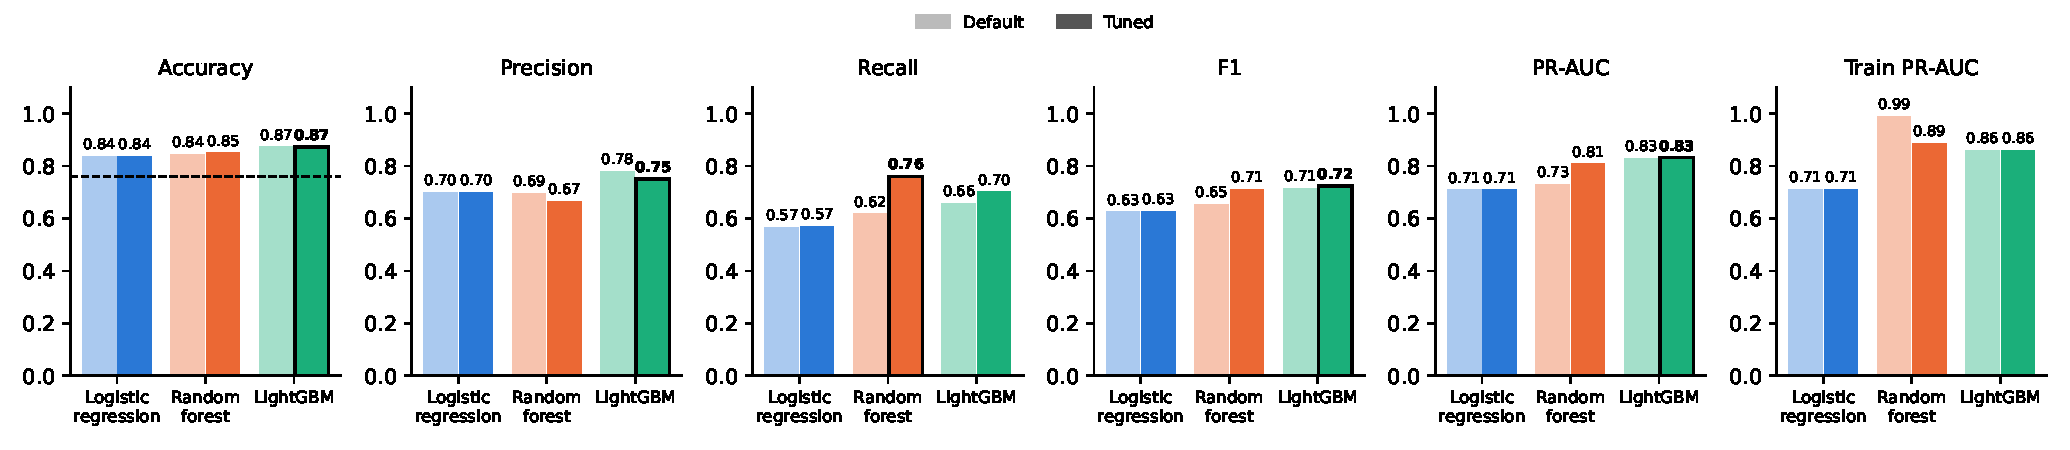
\includegraphics[width=0.9\linewidth]{figures/default_vs_tuned.pdf}
\caption{Default and tuned models (5-fold cross-validation). Left: cross-validated and
training PR-AUC; the gap between the two shows overfitting. Right: precision and recall
at the threshold of 0.5.}
\label{fig:tuned}
\end{figure}

\begin{figure}[htbp]
\centering
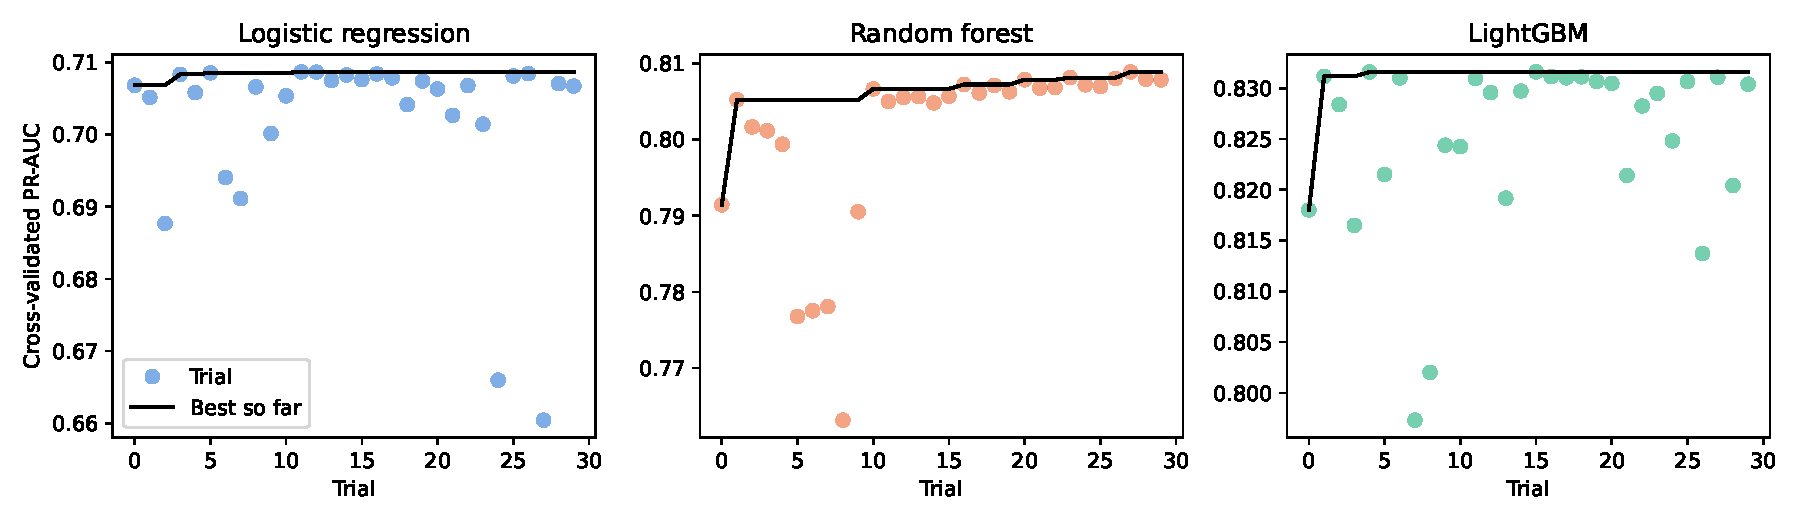
\includegraphics[width=\linewidth]{figures/optuna_history.pdf}
\caption{Cross-validated PR-AUC of each Optuna trial. The black line is the best value
found so far.}
\label{fig:optuna}
\end{figure}

\paragraph{Logistic regression.}
Tuning brings no gain: the PR-AUC stays at 0.709. Optuna also selects almost no
weighting ($w = 1.02$) and a weak regularisation. This confirms the diagnosis of
Section~\ref{sec:models}: the model does not overfit, and its score is limited by its
linear form, which no hyperparameter can change.

\paragraph{Random forest.}
The random forest benefits most from tuning: its PR-AUC rises from 0.731 to 0.809
(Figure~\ref{fig:tuned}, left). The gap between training and cross-validation falls from
26 points (0.991 against 0.731) to 8 points (0.886 against 0.809). The tuned trees are
shallower (depth 18) and keep at least 3 observations per leaf, so they no longer learn
individual training rows, as expected in Section~\ref{sec:models}. Optuna also selects
25 features per split, far above the default of 7.

\paragraph{LightGBM.}
The PR-AUC barely changes (0.830 to 0.832): the default settings were already close to the
best ones. The tuned model uses very small trees (9 leaves) with many boosting steps, and
its gap between training and cross-validation stays at about 3 points (0.861 against
0.832). The main change is at the default threshold: with $w = 1.31$, recall rises from
0.658 to 0.702, while precision falls from 0.781 to 0.750, and F1 improves slightly.

\paragraph{Role of the class weight.}
Optuna selects weights between 1.02 and 2.05, below full rebalancing (3.18).
Figure~\ref{fig:tuned} (right) shows the effect of $w$: the larger the weight, the more
recall rises and precision falls. The random forest has the largest weight and the
largest gain in recall (0.618 to 0.761), while the logistic regression, with $w$ close to
1, does not change. On the other hand, $w$ has little effect on PR-AUC, which does not
depend on the threshold. For example, the eight best LightGBM trials all reach a PR-AUC
of 0.831 or 0.832, with $w$ between 1.18 and 1.99. The selected value of $w$ is therefore
one of many equivalent choices, and should be read with caution.

\paragraph{Number of trials.}
Figure~\ref{fig:optuna} shows that the scores level off quickly. For the logistic
regression and LightGBM, the trials after the first 15 improve the best PR-AUC by less
than 0.001. The random forest still improves slightly after 15 trials (+0.002), and its
best trial is one of the last ones. More trials could therefore add a little to its
score, but this gain is small compared with its gap to LightGBM (2.3 points). A budget
of 30 trials is therefore sufficient to compare the three models.

\paragraph{Choice of the model.}
LightGBM remains the best model after tuning (PR-AUC of 0.832, against 0.809 for the
random forest and 0.709 for the logistic regression), so it is our final model. This
choice relies on cross-validation only. Note that the best cross-validated score is
slightly optimistic: the best of 30 trials is chosen and scored on the same folds. The
unbiased estimate of the final model will come from the untouched test set, which is only
used in the final evaluation.

%=====================================================================
\section{Experiment Tracking}
\label{sec:tracking}
%=====================================================================
All tuning runs are logged with MLflow, in a local database (\texttt{mlflow.db}). The
experiment contains 94 runs, organised as follows:
\begin{itemize}
\item \textbf{One run per model} (3 runs). It stores the best hyperparameters and the
cross-validated metrics of the best trial, and the file \texttt{best\_params.json} as an
artifact.
\item \textbf{One run per trial} (90 runs), nested in the run of its model. Each one
stores the hyperparameters of the trial, including $w$, and all the metrics of
Section~3.1: precision, recall, F1, ROC-AUC and PR-AUC in cross-validation, the standard
deviation of PR-AUC across folds, and the training PR-AUC.
\item \textbf{One summary run}. It stores, as artifacts, the comparison table
(\texttt{tuning\_results.csv}), the best hyperparameters of the three models, and
Figures~\ref{fig:tuned} and~\ref{fig:optuna}.
\end{itemize}

This tracking makes every result of Section~\ref{sec:tuning} traceable: any trial can be
found with its exact settings and scores, and the trials can be compared in the MLflow
interface. The best hyperparameters are also saved in \texttt{results/best\_params.json},
which the next steps use to rebuild the final model.

%=====================================================================
\begin{thebibliography}{9}
\bibitem{kohavi1996} R.~Kohavi. Scaling up the accuracy of naive-Bayes classifiers: A decision-tree hybrid. In \emph{Proceedings of KDD}, 1996.
\bibitem{rubin1976} D.~B.~Rubin. Inference and missing data. \emph{Biometrika}, 63(3):581--592, 1976.
\bibitem{saito2015} T.~Saito and M.~Rehmsmeier. The precision-recall plot is more informative than the ROC plot when evaluating binary classifiers on imbalanced datasets. \emph{PLoS ONE}, 10(3):e0118432, 2015.
\end{thebibliography}

\appendix
\section{Additional Figures}
\label{app:figures}

\begin{figure}[htbp]
\centering
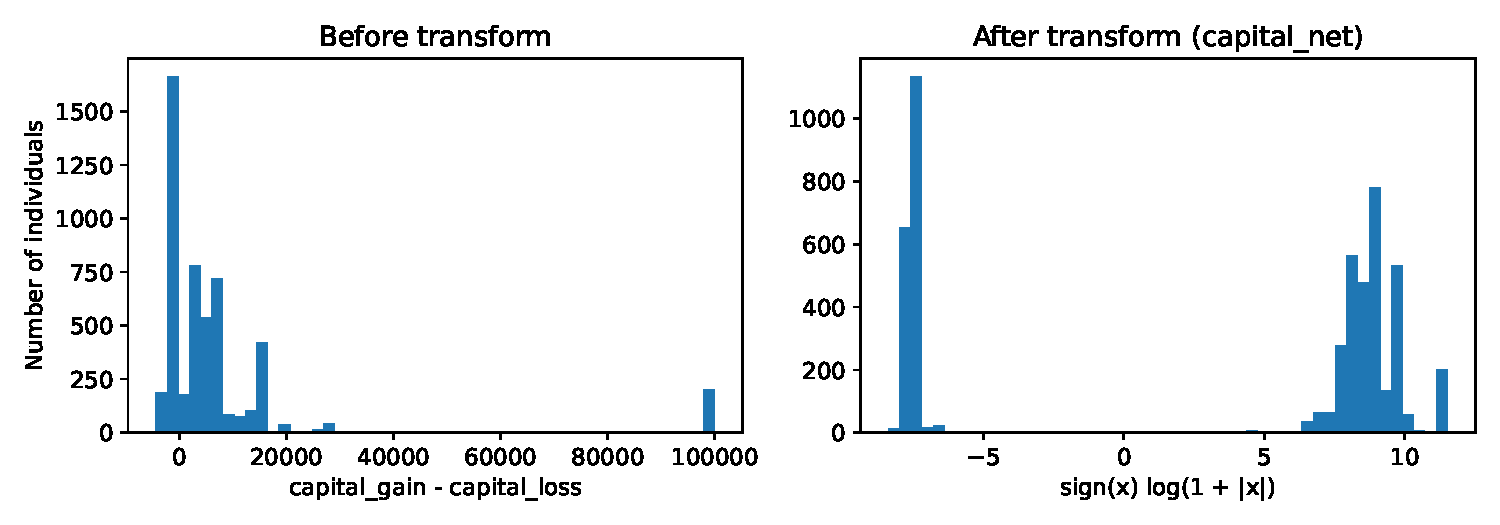
\includegraphics[width=0.9\linewidth]{figures/capital_net_transform.pdf}
\caption{Non-zero net capital income (capital gain minus capital loss, training set)
before and after the signed log transform. The transform compresses the long right tail;
the two groups after the transform correspond to losses (negative values) and gains.}
\label{fig:capital}
\end{figure}

\end{document}